% !TEX encoding = UTF-8 Unicode
% 予備審査レジュメ 案A(空間熱干渉の筋)で作り直した版・2 ページ(11/25、Claude 下書き → レオが読んで直す)。前の版は resume.tex(4 ページ)・resume2.tex(2 ページ)
% 図をページ幅で入れるため multicols ではなく twocolumn にした(11/22)
% ヘッダーは先輩(2025年度 7307)の「創造工学専攻 情報工学コース / 年度 特別研究 2 審査会」に合わせた
% ビルド:thesis/resume/ で latexmk resume.tex → build/resume.pdf
\documentclass[10pt,uplatex,dvipdfmx,twocolumn]{jsarticle}

% 描画・色関連
\usepackage[dvipdfmx]{graphicx}
\usepackage[dvipdfmx]{xcolor}
\usepackage{here}

% レイアウト調整関連
\usepackage{geometry}
\usepackage{setspace}
\usepackage{fancyhdr}
\usepackage{float}

% 数式関連
\usepackage{amsmath}
\usepackage{amssymb}
\usepackage{mathtools}
\usepackage{bm}

% 表・リスト関連
\usepackage{booktabs}
\usepackage{enumerate}

% テキスト装飾関連
\usepackage{url}

% キャプション関連
\usepackage{caption}
\usepackage{subcaption}

\graphicspath{{figures/}{../figures/}{../../experiments/}}
\geometry{a4paper, left=20mm,right=20mm,top=20mm,bottom=20mm}

\definecolor{tmcitblue}{cmyk}{0.86,0.91,0,0.04}
\pagestyle{fancy}
\fancyhf{}
\lhead{\color{tmcitblue}\footnotesize 東京都立産業技術高等専門学校}
\rhead{\color{tmcitblue}\footnotesize 専攻科 情報工学コース\\2026 年度特別研究Ⅱ予備審査会}
\lfoot{\color{tmcitblue}\footnotesize Tokyo Metropolitan College of Industrial Technology}
\cfoot{\thepage}
\renewcommand{\headrulewidth}{0.0pt}
\setlength{\headheight}{20.2781pt}
% ページ幅の図(figure*)をページの上に2つまで置けるように
\setcounter{dbltopnumber}{3}
\renewcommand{\dbltopfraction}{0.85}
\renewcommand{\dblfloatpagefraction}{0.85}
\renewcommand{\textfraction}{0.1}

% 節と図の前後の空きを詰める
\setlength{\textfloatsep}{8pt plus 2pt minus 2pt}
\setlength{\dbltextfloatsep}{8pt plus 2pt minus 2pt}
\captionsetup{skip=4pt}
\makeatletter
\renewcommand{\section}{\@startsection{section}{1}{\z@}{0.6\Cvs \@plus.3\Cdp}{0.3\Cvs}{\normalfont\large\headfont\raggedright}}
\renewcommand{\subsection}{\@startsection{subsection}{2}{\z@}{0.3\Cvs \@plus.2\Cdp}{0.1\Cvs}{\normalfont\normalsize\headfont}}
\makeatother

\begin{document}
\setstretch{1.00}
\twocolumn[{%
\centering
\Large{エッジマイクロクラスタにおける空間熱干渉を考慮した熱抑制手法の研究}\\
\vspace{6pt}
\large{7303 鈴木黎映}\\
\large{指導教員 知念賢一教授}
\vspace{10pt}
}]
% 赤字【】は結果待ち・要確認
\newcommand{\TBD}[1]{\textcolor{red}{【#1】}}

\section{はじめに}
データセンタでは、サーバの排熱が別のサーバの吸気側に回り込む熱の再循環が、冷却の効率を下げる~\cite{moore,tang}。同じことは、小型の計算機を棚や箱に密に並べたエッジのマイクロクラスタ~\cite{iridis}でも起こりうる。あるノードの排熱で隣のノードの温度が上がる現象を、本研究では空間熱干渉と呼ぶ。Raspberry Pi 4B(以下、Raspi)は CPU 温度が約 80\,℃ を超えるとクロックを下げ(スロットリング)、処理が遅くなる。ファンを常に回せば温度は下がるが、ファンの寿命は稼働時間で表され~\cite{kim}、騒音にもなる。そのため、スロットリングを避けつつ、ファンの稼働をできるだけ減らしたい。

先行発表~\cite{ipsj}では、空間熱干渉を外部熱影響 $H$ として推定するカルマンフィルタを提案した。そこでは、密閉した容器の中で隣のノードの負荷だけでアイドルのノードが約 12\,℃ 上がった。一方、開いたラックに横に並べた予備的な測定では 0.5\,℃ 未満であった。空間熱干渉は配置によって大きく変わるが、どのような配置で起こるのかは測られていなかった。本研究では、まず、空間熱干渉がどの条件で起こるかを、位置関係(上下・左右・斜め)、発熱量、囲いの有無を変えて実機で測る。次に、空間熱干渉を推定に取り込んだ予測とファン制御が、干渉の起こる条件と起こらない条件でどう働くかを評価する。

\section{関連研究}
データセンタでは、熱の再循環を考慮した負荷の配置~\cite{moore,tang}が、計算機の内部では温度を予測して先回りする熱管理~\cite{zanini,coskun,yeo}が研究されている。これらは部屋全体か 1 台の内部を対象としており、密に並べた小型の計算機の間で熱がどの程度伝わるかを実測したものではない。

\section{提案手法}
温度を室温からの上昇分 $\theta_t = T_t - T_{\mathrm{amb}}$ で表し、熱 RC モデルを 5 秒ごとに離散化する。
\begin{gather}
  \theta_{t+1} = a\,\theta_t + b\,u_t + c\,H_t + e\,f_t + d \\
  H_{t+1} = \rho\,H_t + (1-\rho)\,z_t
\end{gather}
$u_t$ は CPU 使用率、$f_t$ はファンの状態(0/1)、$z_t$ は隣接ノードの温度のアイドル時からの変化分である。$b > 0$ は負荷による加熱、$e < 0$ はファンによる冷却、$c \ge 0$ は外部熱影響 $H_t$ の効きを表す。干渉が起こらない配置では同定すると $c \approx 0$ となり、自ノードだけのモデルに戻るため、干渉の有無を前もって知らなくても同じ手法を使える。$[\theta_t, H_t]^\top$ をカルマンフィルタで推定し(隣の温度が急に変わると $H$ のプロセスノイズを大きくする)、今の負荷が続きファンは OFF のままと仮定して、30 秒先の温度と標準偏差 $\sigma_t$ を予測する。
\begin{equation}
  M_t = \alpha\,\sigma_t + \delta,\qquad T_{\mathrm{safe}} = T_{\mathrm{limit}} - M_t
\end{equation}
$\alpha = 2$、$\delta = 0.5$\,℃、$T_{\mathrm{limit}} = 80$\,℃ とし、予測温度が $T_{\mathrm{safe}}$ を超えたらファンを ON にする(最小 ON 時間 30 秒、OFF は 1\,℃ のヒステリシス)。

\section{実験}
\begin{figure}[tb]
  \centering
  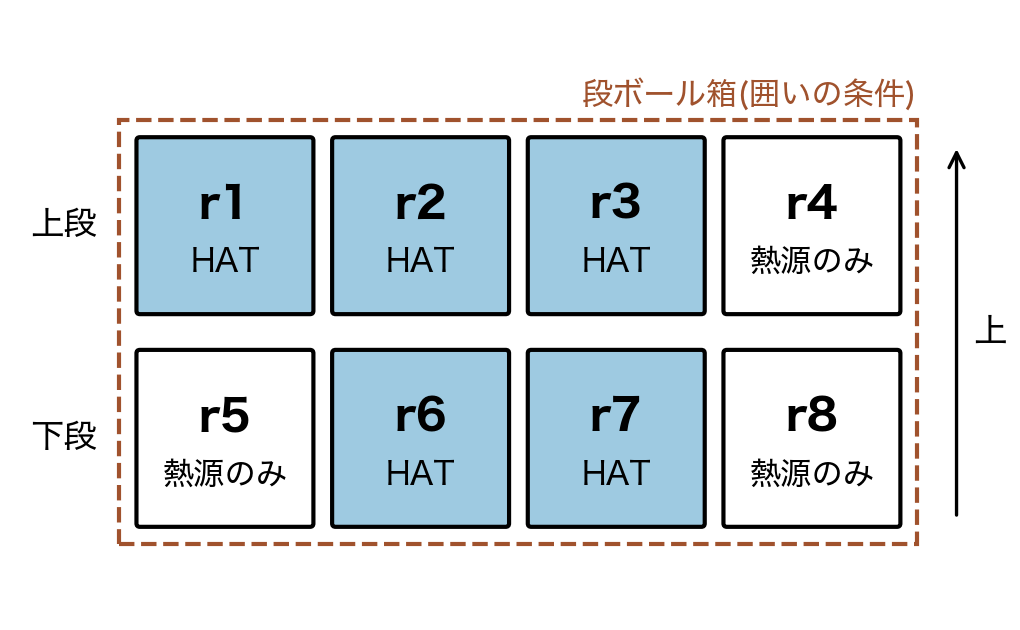
\includegraphics[width=0.78\columnwidth]{fig_rack_layout.png}
  \caption{ラックの配置(ポート側から見た図)。網掛けは PoE+ HAT(ファン付き)のあるノード}
  \label{fig:layout}
\end{figure}
Raspi 8 台を 2 段 × 4 列のラックに縦向きに固定した(図~\ref{fig:layout})。5 台は PoE+ HAT のファンを制御用 PC から ON/OFF し、残りの 3 台はファンのない熱源とした。8 台すべての温度・クロックなどを 1 秒ごとに集め、部屋とラック(箱)の上部・正面の気温も記録した。1 台の消費電力はアイドルで約 2.4\,W、2 コアの負荷で約 3.8\,W である。

確かめることは、空間熱干渉がどの位置関係・発熱量・囲いの有無で起こるか(Q1)、冷やすときにも干渉が影響するか(Q2)、干渉が起こる条件で $H$ を持つ予測が当たるか(Q3)、予測に基づくファン制御で稼働を減らせるか(Q4)である。囲いは、なしと、段ボール箱(約 8\,L。上・左右・後ろを覆い、正面と下は開いている)をラック全体にかぶせた状態の 2 通りとした。2 コアの負荷 10 分と休み 12 分を 1 ブロックとし、r6 だけ・r7 だけ・下段 4 台・8 台すべてに負荷をかけた。Q2 では、ファンの風で排熱が隣に運ばれるか(r6 のファンを ON にして負荷)と、隣が熱いと冷え方が弱くなるか(r2 のファンを ON にしたときの冷え方を、隣がアイドルのときと負荷のときで比べる)を見た。負荷をかけていないノードの上昇(室温の変化を引く)が 1\,℃ 以上なら「干渉あり」とし、条件と基準は測定の前に決めた。Q4 は、横に 3 台並べた予備実験で、20 分の負荷のパターンを 5 条件で 3 巡行って評価した。

\section{結果}
\begin{table}[tb]
  \centering
  \caption{負荷をかけていないノードの上昇(℃、室温の変化を引いた値)}
  \label{tab:pattern}
  \footnotesize\setlength{\tabcolsep}{2pt}
  \begin{tabular}{@{}lrr@{}}
    \toprule
    負荷 → 見るノード & 開いた状態 & 箱 \\
    \midrule
    真上(r6→r2, r7→r3) & $+0.1$, $+2.0$ & $-0.5$, $+0.5$ \\
    横(r6→r7, r7→r6) & $-1.4$, $+1.3$ & $-0.2$, $-0.2$ \\
    斜め上(r6→r1・r3, r7→r2) & $-0.3$, $-1.5$, $+1.0$ & $-0.1$, $-0.4$, $0.0$ \\
    離れた位置(r7→r1) & $+0.4$ & $+0.1$ \\
    下段 4 台 → 上段 r1〜r4 & $+0.6$〜$+1.4$ & $+0.1$〜$+1.8$ \\
    \bottomrule
  \end{tabular}
\end{table}
\begin{figure}[tb]
  \centering
  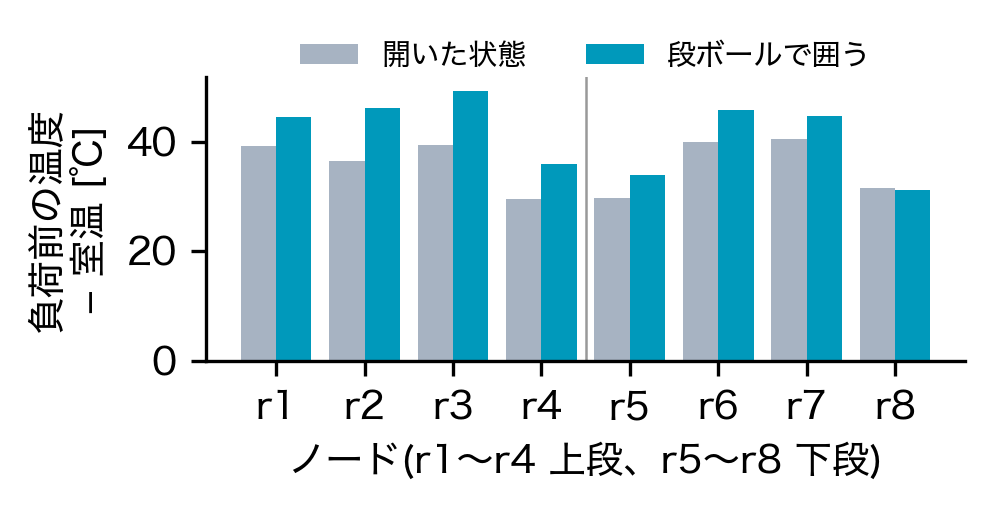
\includegraphics[width=0.95\columnwidth]{fig_pattern_idle.png}
  \caption{負荷をかける前の温度と室温の差(開いた状態と段ボール箱)}
  \label{fig:idle}
\end{figure}
Q1 の結果を表~\ref{tab:pattern}に示す。開いた状態では、部屋の温度の変化による揺れ(約 $\pm 1.5$\,℃)に埋もれ、向きによって結果がそろわなかった。揺れの小さい箱では、どの位置関係でも $\pm 0.5$\,℃ 以内であった。一方、図~\ref{fig:idle}に示すように、囲うだけで負荷の前の温度は 5〜10\,℃ 高くなり、8 台に同時に負荷をかけると、箱ではファン付きの 5 台がすべて 83\,℃ に達した(開いた状態でも 4 台が 80〜83\,℃)。Q2:隣が熱くても、r2 のファンを ON にしたときの下がり幅は同じ(17〜19\,℃)で、r6 のファンの風による隣の上昇もなかった。Q3:上段の 30 秒先の平均絶対誤差は、自ノードだけのモデルの 0.64(開いた状態)・0.84\,℃(箱)に対し、$H$ を持つモデルで 0.39・0.44\,℃ であった。箱では、正面の気温を室温として使う自ノードだけのモデルも 0.41\,℃ で、$H$ と同じ精度であった。

Q4 では、予測を用いる 2 方式としきい値方式(75\,℃ で ON、70\,℃ で OFF)は、9 回すべてで 80\,℃ を超えなかった。提案手法のファン稼働率は 38\% で、常時 ON より約 6 割少なく、干渉のない配置で $c \approx 0$ となっても壊れずに働いた。ただし、しきい値方式(40\%)との差はほぼなかった。PoE+ HAT のファンは 5 秒以内に効き始めるため、温度が上がってから回しても間に合い、予測の利点が小さいと考えられる。

\section{考察とまとめ}
空間熱干渉を「ほかのノードの発熱で自ノードの温度が上がること」とすると、1 台の排気が隣を直接温める経路は位置関係によらず 1\,℃ 未満で、考慮が要るのは、囲いやラックの空気に熱が溜まる経路(囲いの閉じ方と同時に動く台数)であった。先行発表の約 12\,℃ の上昇も、密閉した小さな容器で溜まる経路が効いた結果と考えられる。箱では、箱の中の気温を使うモデルが $H$ と同じくらい当たったことから、測定前に決めた解釈に従い、$H$ の役割は「箱の中に温度計がないときに、隣の温度からその昇温を推定する」ことと考える。開いた状態では、どの気温を使っても $H$ ほど当たらなかった。また、隣が熱くてもファンの効きは弱まらず、干渉は温度の水準を押し上げるだけであったため、速く効く PoE+ HAT のファンでは、干渉のある配置でも予測の利点は出にくい。空間熱干渉を状態として推定するファン制御は、干渉のない配置でも壊れずに働き、80\,℃ を超えずに稼働を約 6 割減らした。今後は、囲いの大きさ・閉じ方と発熱量を変えて溜まる経路が効き始める条件を調べ、干渉が起こる配置でファン制御を評価する。

\section*{先行発表}
本研究の空間熱干渉を考慮した状態推定とマージンの手法は、情報処理学会 システムソフトウェアとオペレーティング・システム研究会で発表した~\cite{ipsj}。

\scriptsize{
\begin{thebibliography}{99}
  \setlength{\itemsep}{0pt}
  \bibitem{moore} J. Moore et al., ``Making Scheduling ``Cool'': Temperature-Aware Workload Placement in Data Centers,'' USENIX ATC, pp.61--74, 2005.
  \bibitem{tang} Q. Tang et al., ``Energy-Efficient Thermal-Aware Task Scheduling for Homogeneous HPC Data Centers,'' IEEE TPDS, Vol.19, No.11, pp.1458--1472, 2008.
  \bibitem{iridis} S. J. Cox et al., ``Iridis-pi: a low-cost, compact demonstration cluster,'' Cluster Computing, pp.349--358, 2014.
  \bibitem{kim} S. J. Kim, A. Claassen, ``How to Evaluate Fan Life,'' Electronics Cooling, 1996.
  \bibitem{ipsj} 鈴木 黎映, 知念 賢一, ``空間熱干渉を考慮した状態推定に基づく動的熱マージン制御手法,'' 情報処理学会研究報告, Vol.2026-OS-171, No.3, 2026.
  \bibitem{zanini} F. Zanini et al., ``Multicore Thermal Management with Model Predictive Control,'' Proc. ECCTD, pp.711--714, 2009.
  \bibitem{coskun} A. K. Coskun et al., ``Proactive Temperature Management in MPSoCs,'' Proc. ISLPED, 2008.
  \bibitem{yeo} I. Yeo et al., ``Predictive Dynamic Thermal Management for Multicore Systems,'' Proc. DAC, pp.734--739, 2008.
\end{thebibliography}
}
\end{document}
